\documentclass[aps,prl,twocolumn,superscriptaddress,amsfont,graphicx,preprintnumbers]{revtex4-1}
\usepackage{color,graphicx,epsfig}
\usepackage{ifpdf}
\usepackage{amsmath}
\usepackage{bm}
\usepackage{color}
\usepackage[english]{babel}
\usepackage{booktabs}
\usepackage{graphicx}
\usepackage{amsfonts}
\usepackage{amssymb}
\usepackage{hyperref}
\usepackage{slashed}
\usepackage{url}
\usepackage{array}
\usepackage{enumerate}


\bibliographystyle{apsrev4-1}

\definecolor{nicered}{rgb}{0.7,0.1,0.1}
\definecolor{nicegreen}{rgb}{0.1,0.5,0.1}
\hypersetup{colorlinks,citecolor= nicegreen,linkcolor= nicered}

% macros
\newcommand{\M}{\mathcal{M}}
\newcommand{\xgb}{\texttt{XGBoost}~}
\newcommand{\lgbm}{\texttt{LightGBM}~}
\newcommand{\openl}{\texttt{OpenLoops}~}
\newcommand{\tenr}{{\it`10~regions'}~}
\newcommand{\oner}{{\it`1~region'}~}
\newcommand{\msq}{\langle\left|\mathcal{M}\right|^2\rangle}
\newcommand{\cth}{\cos\theta}
\newcommand{\mz}{m_Z}
\newcommand{\ptx}{p_{T,\text{cut}}}
\newcommand{\dmsqdrts}{d\msq/d\sqrt{\hat{s}}}
\newcommand{\mcM}{\mathcal{M}}
%
\definecolor{Red}{rgb}{1.,0.,0.}
\definecolor{Blu}{rgb}{0.1,0.3,0.9}
\newcommand{\red}[1]{{\color{Red}{#1}}}
\newcommand{\blu}[1]{{\color{Blu}{#1}}}
\newcommand{\fady}[1]{\red{\bf [FB: #1]}}
\newcommand{\comm}[1]{\blu{\bf [FB: #1]}}
%
\newcommand{\shat}{\hat{s}}
\newcommand{\rtshat}{\sqrt{\shat}}
%
\newcommand{\MKL}{\mathcal{M}^{[X_r]}_{\kappa\lambda}}
\newcommand{\MAkl}[2]{\mathcal{M}^{[A_#1]}_{#2}}
\newcommand{\MBkl}[2]{\mathcal{M}^{[B_#1]}_{#2}}
\newcommand{\MCkl}[2]{\mathcal{M}^{[C_#1]}_{#2}}

\graphicspath{{./figs/}}
%
%%%%%%%%%%%%%%%%%%%%%%%%%%%%%%%%%%%%%%%%%%
\begin{document}
%%%%%%%%%%%%%%%%%%%%%%%%%%%%%%%%%%%%%%%%%%
\def\DESY{DESY, Notkestra{\ss}e 85, 22607 Hamburg, Germany}
\def\PSI{Paul Scherrer Institut, Forschungsstra{\ss}e 111, 5232 Villigen PSI, Swizerland}
\def\Zurich{Physik-Institut,  Universit{\"a}t  Z{\"u}rich,  Winterthurerstrasse  190,  CH-8057  Z{\"u}rich,  Switzerland}
%%%%%%%%%%%%%%%%%%%%%%%%%%%%%%%%%%%%%%%%%%
\preprint{DESY 20-, UZH -, PSI - }
%%%%%%%%%%%%%%%%%%%%%%%%%%%%%%%%%%%%%%%%%%
%\title{\boldmath Machine Learning $q q \to VV \to 4 \ell$ amplitudes at NNLO ($10^4$ $\times$ faster)}
%\title{\boldmath ``Slow" terms in $q q \to 4 \ell$ at NNLO ($10^4$ $\times$ faster) with Machine Learning}
%\title{\boldmath Speeding up the ``slow" terms in $q q \to 4 \ell$ at NNLO with Machine Learning}
%\title{\boldmath Machine Learning the ``slow" terms in $q q \to 4 \ell$ at NNLO ($10^4$ $\times$ faster)}
%\title{\boldmath Machine Learning the ``slow" terms in $q q \to 4 \ell$ at NNLO}
%\title{\boldmath  Faster $q q \to 4 \ell$ at NNLO with Machine Learning}
\title{\boldmath  A simple way to speed up $q q \to 4 \ell$ generation at NNLO}
%%%%%%%%%%%%%%%%%%%%%%%%%%%%%%%%%%%%%%%%%%
\author{Fady Bishara}
\email[Electronic address:]{fady.bishara@desy.de}
\affiliation{\DESY}
\author{Marc Montull} 
\email[Electronic address:]{marc.montull@gmail.com}
\affiliation{\PSI}\affiliation{\Zurich}
%%%%%%%%%%%%%%%%%%%%%%%%%%%%%%%%%%%%%%%%%%
\begin{abstract} 
We show that Machine Learning regressors can be used to infer the "slow" pieces of the $qq\to4 \ell$ NNLO amplitude in ${\cal O}(10^{-5})$ seconds (as opposed to the 10 seconds one requires to compute them exactly). This speed up can be achieved while keeping the errors on the NNLO correction below $10\%$ and the error on the total NNLO amplitude below $0.1\%$. The speed up of the "slow" terms in the NNLO correction results in an increase of ${\cal O}(10^4)$ in the NNLO correction to the $qq \to 4 \ell$ amplitude, bringing it down to the millisecond range. This improvement can be done relatively easily since there are many regions in the PS where the "slow" pieces are sub-leading and therefore one can infer those regions less precisely without a large impact on the full NNLO correction.
%We show that Machine Learning regressors can be used to infer the values of the ``slow" 
%(tree $\times$ 2-loop ) pieces which appear in the double resonant $q q' \to VV' \to 4\ell$ amplitudes for $V,V' = Z, W, \gamma$,  with a relatively small error and with a speed \red{$10^4$} times faster than the specialized software currently used to compute them. In order to do this, we train the ML regressors on the $2 \to 2$ sub-amplitudes which reduces the number of variables of the functions we need to predict (from 8 to 4).
%and allows the trained regressors to be used for any given $V, \, V'$ amplitude. 
%We use the various symmetry relations between the different classes of diagrams to reduce the number of regressors to train. As a proof of concept we show that we are able to reproduce the non-trivial tree $\times$ 2-loop terms for the process $q q' \to WZ(\gamma^*) \to e^+ e^- \mu \nu_\mu$ with errors below \red{$7 \%$} requiring a disk size below \red{2 Gb}.
\end{abstract}
%%%%%%%%%%%%%%%%%%%%%%%%%%%%%%%%%%%%%%%%%%
\maketitle
%%%%%%%%%%%%%%%%%%%%%%%%%%%%%%%%%%%%%%%%%%
\section{Introduction}

Need precision for ILC, FCC-ee and CLIC, due to high luminosity, hence need to go to N(N)LO. Problem with time consuming MC generation. Machine learning can solve this, both with phase space integration \cite{} and more recently some works trying to make the evaluation of amplitudes to be faster \cite{Bishara:2019iwh,Badger:2020uow}. 
\medskip

A lot of work relating diboson at high $\sqrt{s}$ and the search for new physics
\cite{Falkowski:2015jaa,Butter:2016cvz,Azatov:2017kzw,Franceschini:2017xkh,Grojean:2018dqj,Bellazzini:2018paj,Biekotter:2018rhp,Banerjee:2018bio,Grojean:2018dqj, Baglio:2018bkm,Azatov:2019xxn, Brehmer:2019gmn,Liu:2019vid, Banerjee:2019pks,Banerjee:2019twi,Chiu:2019ksm,Baglio:2019uty, Bishara:2020vix, Baglio:2020oqu,Bishara:2020pfx,Bishara:2020vix}. \red{Motivate why we choose WZ from BSM most important channel}

\begin{figure*}
\begin{equation}
\def\arraystretch{2}
\begin{array}{lcccccc}
\toprule
& A & B & C & F_W & F_Z & F_\gamma \\
\hline
&&&&&&\\[-0.7cm]
u_L \bar{d}_L \to W^+Z       & \dfrac{-3+2 \, e \, s_W^2}{6 c_W s_W^2 \sqrt{2}}& \dfrac{3-4 \, e \, s_W^2}{6 c_W s_W^2 \sqrt{2}} & 0 &   \dfrac{\pm c_W}{s_W}  & 0 & 0\\
u_L \bar{d}_L \to W^+\gamma  & \dfrac{-e}{s_W 3 \sqrt{2}}  & X & 0 &  \dfrac{\pm c_W}{s_W} & 0 & 0\\[0.2cm]
\hline
q_L \bar{q}_L \to W^+W^-             & X & X & 0 & 0 &  \dfrac{\pm c_W}{s_W}  & \pm 1\\
\hline
q_R \bar{q}_R \to W^+W^-             & X & X & 0 & 0 &  \dfrac{\pm c_W}{s_W}  & \pm 1\\
\hline
q_L \bar{q}_L \to ZZ & X & X & 0 & 0 & 0 & 0\\
q_L \bar{q}_L \to Z\gamma & X & X & 0 & 0 & 0 & 0\\
q_L \bar{q}_L \to \gamma\gamma & X & X & 0 & 0 & 0 & 0\\
\hline
q_R \bar{q}_R \to ZZ & X & X & 0 & 0 & 0 & 0\\
q_R \bar{q}_R \to Z\gamma & X & X & 0 & 0 & 0 & 0\\
q_R \bar{q}_R \to \gamma \gamma & X & X & 0 & 0 & 0 & 0\\
\hline
%(\gamma)Z(\gamma)
\bottomrule
\end{array}
\end{equation}
\caption{couplings for blabla}
\end{figure*}

In previous work \cite{Bishara:2019iwh} we showed that \xgb can speed up the on loop $gg \to ZZ$ amplitude squared by a factor $\sim 10^3$ with errors in the double differential distribution below $\lesssim 1 \%$. Here we continue that program by studying a more interesting and challenging process like $q q \to VV \to 4 \ell$.
%\medskip

It is advantageous to separate the helicity amplitudes with intermediate, off-sheel, vector bosons using the completeness relations for the polarization vectors into production and decays helicity amplitudes for three reasons:
\begin{enumerate}
    \item this allows us to fit a 4d rather than 8d phase-space,
%    \item for the production amplitude, fitting the three classes of diagrams separately allows us to fit one function for any combination of $V_1$ and $V_2$ where $V\in{W,Z,\gamma}$ \red{MM: not sure, what about processes where only the A and C classes contribute? (i.e. $WW$ and $Z \gamma$(?))},
   \item Naively, the  $2 \to 2$ helicity sub-amplitudes are well behaved function since one expects the point to point ``j-factors" to be rather flat. This is more intutitive than opposition to the form factors $A_i$, can be much more intuitively and therefore, easily, normalized to reduce the error in the fit. We can fit flatter functions 
   \red{(we should plot the ratios, aka the helicity amplitude ``j-factors" for helamps, and also for the A's (in the Appendix / supplemental material)}. Nonetheless there could be better functioins to fit, which we leave for future work.
   
   \item \red{Anything else?}
   
   % \item helicity amplitudes, as opposed to the form factors $A_i$, can be much more intuitively and therefore, easily, normalized to reduce the error in the fit. We can fit flatter functions \red{(we should plot the ratios, aka the helicity amplitude ``j-factors" for helamps, and also for the A's (in the Appendix / supplemental material)}. Nonetheless there could be better functioins to fit, which we will study in future work.
\end{enumerate}
We will discuss these three points in turn.
\medskip

{\bf The main goal of this work} is to speed up the evaluation of the ``slow" 2-loop $\times$ tree amplitudes in massless QCD by using ML regressors to predict them. Notice that not all these amplitudes are ``slow", since some of them are of the form (tree level amplitude $\times$ form factor) where the form factor can be readily evaluated.

\red{How to be sure that there are no large cancellations between the ``slow" terms we fit and the rest we don't when computing at least the total NNLO part of the amplitude.}

\section{Slow 2-loop amplitudes}

The squared amplitude of the $qq\to4\ell$ process can be perturbatively expanded in $\alpha_s$ at NNLO as follows
\begin{equation}
\begin{aligned}
|\mcM_{2 \to 4}|^2 &= |\mcM_{(0)}|^2 + \left(\frac{\alpha_s}{2\pi} \right) \, 2 \Re[\mcM_{(0)}^* \mcM_{(1)}]  \\
&+\left(\frac{\alpha_s}{2\pi} \right)^2 \left(|\mcM_{(1)}|^2 + 2 \Re[\mcM_{(0)}^* \mcM_{(2)}]. \right) \,.
\label{eq:amplitude}
\end{aligned}
\end{equation}
%\langle \mcM|\mcM\rangle = \langle \mcM^{(0)}|\mcM^{(0)}\rangle + \frac{\alpha_s}{2\pi} \langle \mcM^{(0)}|\mcM^{(1)}\rangle 
The NNLO pieces are given by the 1-loop amplitude squared $|M_{(1)}|^2$ and the interference term between the 2-loop and tree amplitudes $2 \Re[\mcM_{(0)}^* \mcM_{(2)}]$. Given that \texttt{OpenLoops} can easily compute the $|M_{(1)}|^2$ term in miliseconds, we will focus on those terms for which each PS point requires $t \lesssim {\cal O}(10)$ seconds to be computed. These correspond to the $2 \Re[\mcM_{(0)}^* \mcM_{(2)}]$ containing diagrams from the classes $A,B,C$ shown in Fig.~\ref{fig:diagrams}.

\red{Subtlety with same sign electrons}

%In this work, we are interested in training ML regressors to predict the slow pieces of the NNLO contribution of Eq.~\ref{eq:amplitude} which require sophisticated software like \texttt{VVamp} \cite{Gehrmann:2015ora}. 

%These are schematically depicted for the 2-loop contirubtions and without final leptons in Fig.~\ref{fig:diagrams} (except class $F$). The trivial pieces that we don't not consider are those whose 1-loop and 2-loop amplitudes can be written as \red{($\mcM_{(0)} \times$ form factor)} which besides those from class $F$ also include diagrams with a Drell-Yan topology where on of the final leptons radiates a gauge boson that decays into two other leptons (for which the QCD correction is just a vertex correction as well).
%where one intermediate gauge bosons splits into a lepton and another gauge boson which subsequently decays into two leptons.

\begin{figure}
    \centering
    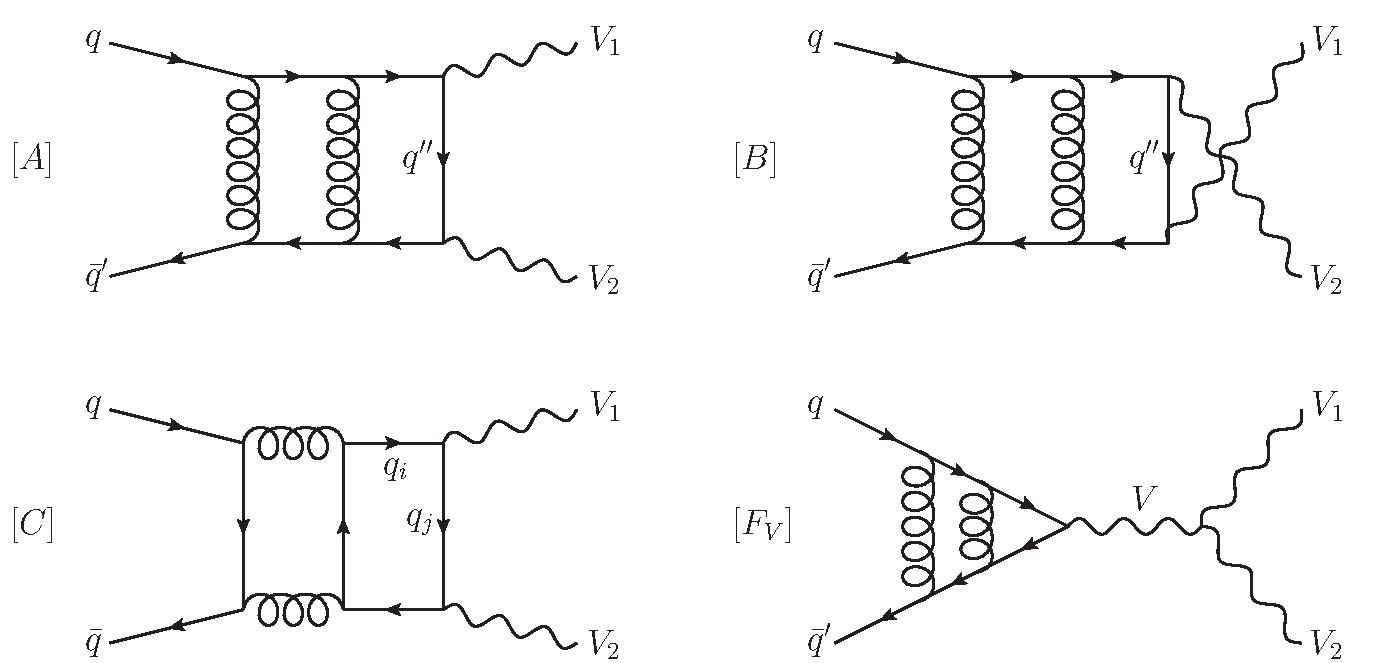
\includegraphics[width=\linewidth]{figs/diagrams.pdf}
    \caption{Representative diagrams contributing to $qq \to 4\ell$. Classes $A$ and $B$ present at tree, 1-loop and 2-loops, while class $C$ only at 2-loops. Diagrams with class $F$ topology are trivial to compute and therefore we do not consider in this work any terms containing them. Figure taken from \cite{Gehrmann:2015ora}.}
    \label{fig:diagrams}
\end{figure}

\begin{boldmath}
\section{$2 \to 2$ sub-amplitues}
\end{boldmath}



Given that all the $qq \to 4\ell$ amplitudes we are interested in are double-resonant, i.e. of the form $q q \to V V$, with each $V$ decaying to $2$ leptons. We divide the full amplitude in $2 \to 2$ helicity sub-amplitudes. We do this for various reasons. First of all our preliminary tests showed that we could achieve more precision by fitting the different sub-amplitudes which are functions of four variables than by fitting the full $2 \to 4$ amplitude which depends on 8 variables.
%. \red{Secondly, by fitting the $2 \to 2$ subamplitudes we can use the same ML regressors for any intermediate combination of gauge bosons $V_3, V_4 = W, Z, \gamma$ (see Eq.~\ref{})}. 
Therefore we rewrite the double-resonant $qq \to VV \to 4\ell$ amplitudes as follows:
%
\begin{equation}
\begin{gathered}
%\begin{aligned}
    \mcM_{2 \to 4} = \, \mcM^{\mu \bar{\mu}}_{2 \to 2} \ P_{\mu\nu} P_{\bar{\mu}\bar{\nu}} J^\nu J^{\bar{\nu}}  \\
    = \sum_{\kappa \lambda , X} \, \left[(\mcM^X_{2 \to 2})^{\mu \bar{\mu}} (\epsilon_\mu^\kappa)^* (\epsilon_{\bar{\mu}}^{\lambda})^* \right] (\epsilon_\nu^\kappa J^\nu) (\epsilon_{\bar{\nu}}^\lambda J^{\bar{\nu}} ) \Delta_{3} \Delta_{4} 
%\end{aligned} \nonumber
\end{gathered}
\end{equation}
%
where in the first line $\mcM^{\mu \bar{\mu}}_{2 \to 2}$ is the $qq \to V_3 V_4$ amplitude, 
%with arbitrary $M_3$ and $M_4$
$P_{\mu \nu}, \, P_{\bar{\mu}\bar{\nu}}$ are the gauge boson propagators and $J^\nu, J^{\bar{\nu}}$ are the lepton currents. In the second line $(\mcM^X_{2 \to 2})$ is the $2 \to 2$ amplitude for each of the classes $X=A, \, B, \, C, \,F_V$ shown in Fig.~\ref{fig:diagrams}, $\Delta_{i} = (p_i^2 - M_i^2)^{-1}$ while $\epsilon_\mu^\lambda$, $\epsilon_\nu^\kappa$ are the intermediate gauge boson polarizations with $\lambda, \, \kappa = \pm, 0$.

%In order to proceed we show in Fig \ref{fig:diagrams} the different class of diagrams $A$, $B$, $C$ and $F$ which are defined by their topology. Note that class $C$ only appears in 2-loop amplitudes, while class $A$ and $B$ appear both at tree level and 1-loop. Class $F$ is 

Note that there are large cancellations between diagrams of different classes. The result of their sum is orders of magnitude smaller than the size of each individual diagram. This is the case between classes $A$ and $B$ for $ZZ/Z\gamma/\gamma\gamma$ and  $A$, $F$ \red{(or $B,F$)} for $WW$ and $WZ/W\gamma$. This fact forbids us to fit each class individually once, and then just re-scale them with appropriate couplings for each proess. Once this advantage is lost we then proceed to train together all the class of diagrams together for each final state. For each $qq \to VV^\prime$ helicity one should train the following combinations of amplitudes
\medskip

\begin{equation}
    \begin{aligned}
    &\mcM^{[P]}_{qq^\prime} = \sum_X g^{[P]}_{qq^\prime} \, \mcM^{[X]}
    \end{aligned}
\end{equation}

where $X \in {A,B,C,F_V}$, $\mcM^{[X]}$ are the $2 \to 2$ helicity amplitudes, and $g^{[P]}_{qq^\prime}$ are given in the following table:




%WZ/W$\gamma$: A, B, F

%ZZ/$\gamma \gamma$: A, B, C

%Z$\gamma$: A, C


\section{Symmetry properties}
%\subsubsection*{Symmetry properties of the helicity amplitudes}

%\subsubsection*{Symmetry relations}
The $q_r\bar{q}_{\bar{r}}\to V_1V_2$ helicity amplitudes $\MKL$ for classes A, B and C have certain symmetry relations under the transformations:
\begin{equation}
\begin{aligned}
&\pi_{12}:=p_{1} \leftrightarrow p_{2} \Rightarrow\{t \leftrightarrow u\} \\ 
&\pi_{34}:=p_{3} \leftrightarrow p_{4} \Rightarrow\left\{t \leftrightarrow u, \quad p_{3}^{2} \leftrightarrow p_{4}^{2}\right\} \,.
\end{aligned}
\end{equation}
These are the following
\begin{equation}
\begin{aligned}
&\MAkl{-}{\kappa\lambda} \xrightarrow{\pi_{12}} (-1)^{N_0} \MBkl{+}{\kappa\lambda}\,, \\
   & \MAkl{-}{\kappa\lambda} \xrightarrow{\pi_{34}} -\MBkl{-}{\lambda\kappa} \\
  & \MAkl{-}{\kappa\lambda}  \xrightarrow{\pi_{12}\circ\pi_{34}} (-1)^{N_0+1} \MAkl{+}{\lambda\kappa} \\
&{\mathcal{M}^{[A(B)_-]}}_{\kappa\lambda} =
    - {\mathcal{M}^{[A(B)_+]}}_{\bar{\kappa}\bar{\lambda}} \\
& \MCkl{-}{\kappa\lambda} \xrightarrow{\pi_{12}} (-1)^{N_0} 
\MCkl{+}{\kappa\lambda}\,, \\
&\MCkl{+}{\kappa\lambda} =\MCkl{-}{\bar\kappa\bar\lambda}  \,, \\
& \MCkl{-}{\kappa\lambda} \xrightarrow{\pi_{34}}
-\MCkl{-}{\lambda\kappa}\,,\\
&\red{class\, F?}
    \end{aligned}
\end{equation}


where the labels $A_\pm$ and $B_\pm$ indicate the class and handedness of the helicity amplitudes (with the sub-indices $+$,$-$ denoting the right and left-handed amplitudes respectively i.e. the eigenvalues of $\gamma_5$). The indices $\kappa,\,\lambda$ are the polarizations of $V_1\,V_2$. In the expressions, $\bar{\kappa}$, $\bar{\lambda}$ correspond to flipping the helicity from $+$ to $-$ and biceversa (while there is no change if  $\bar{\kappa}=0$ or $\bar{\lambda}=0$) while $N_0$ is the number of longitudinal polarizations $\kappa,\lambda$ that equal zero.  

The following transformation are combinations of the previous ones in (A.1)-(A.4), and are useful when inferring the helicity amplitudes fitting the least number of regressors as explained in \red{Sec. X}.

\begin{equation}
\MAkl{-}{\kappa\lambda} \xrightarrow{\pi_{12}} 
    (-1)^{N_0+1} \MBkl{-}{\bar{\kappa}\bar{\lambda}} 
\end{equation}

\begin{equation}
{\mathcal{M}^{[A_-]}}_{\kappa\lambda}  \xrightarrow{\pi_{12} \circ \pi_{34}} 
    (-1)^{N_0} {\mathcal{M}^{[A_-]}}_{\bar{\lambda} \bar{\kappa}} 
\end{equation}

\red{Need to write the symmetry properties that we used (the useful ones) for each of the combinations that we say we can fit}
\medskip

WW:

WZ/W$\gamma$:

ZZ/$\gamma \gamma$:

$Z\gamma$:


%%%%%%%%%%%%%%%%%%%%%%%%%%%%%%%%%%%%%%%%%%%%%%%%%
\section{Results}
\label{sec:Results}

In this section we show ...

\begin{figure}
    \centering
    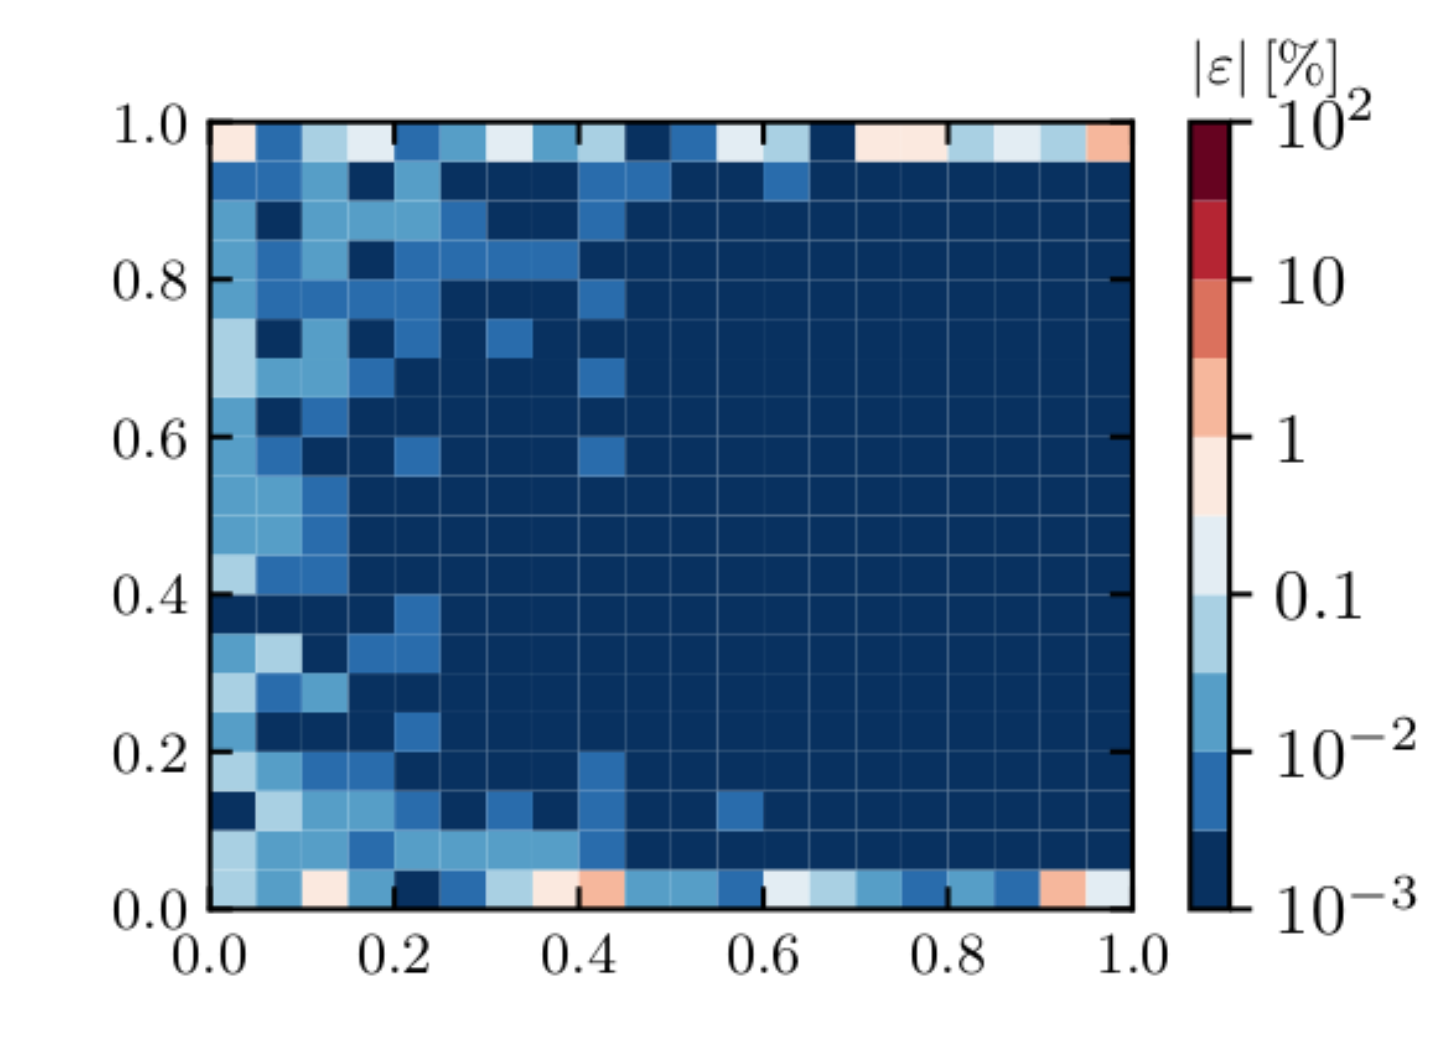
\includegraphics[width=\linewidth]{figs/sqrts_costh.png}
    \caption{bla bla \red{put correct plot}}
    \label{fig:sqrts_costh}
\end{figure}

\begin{figure}
    \centering
    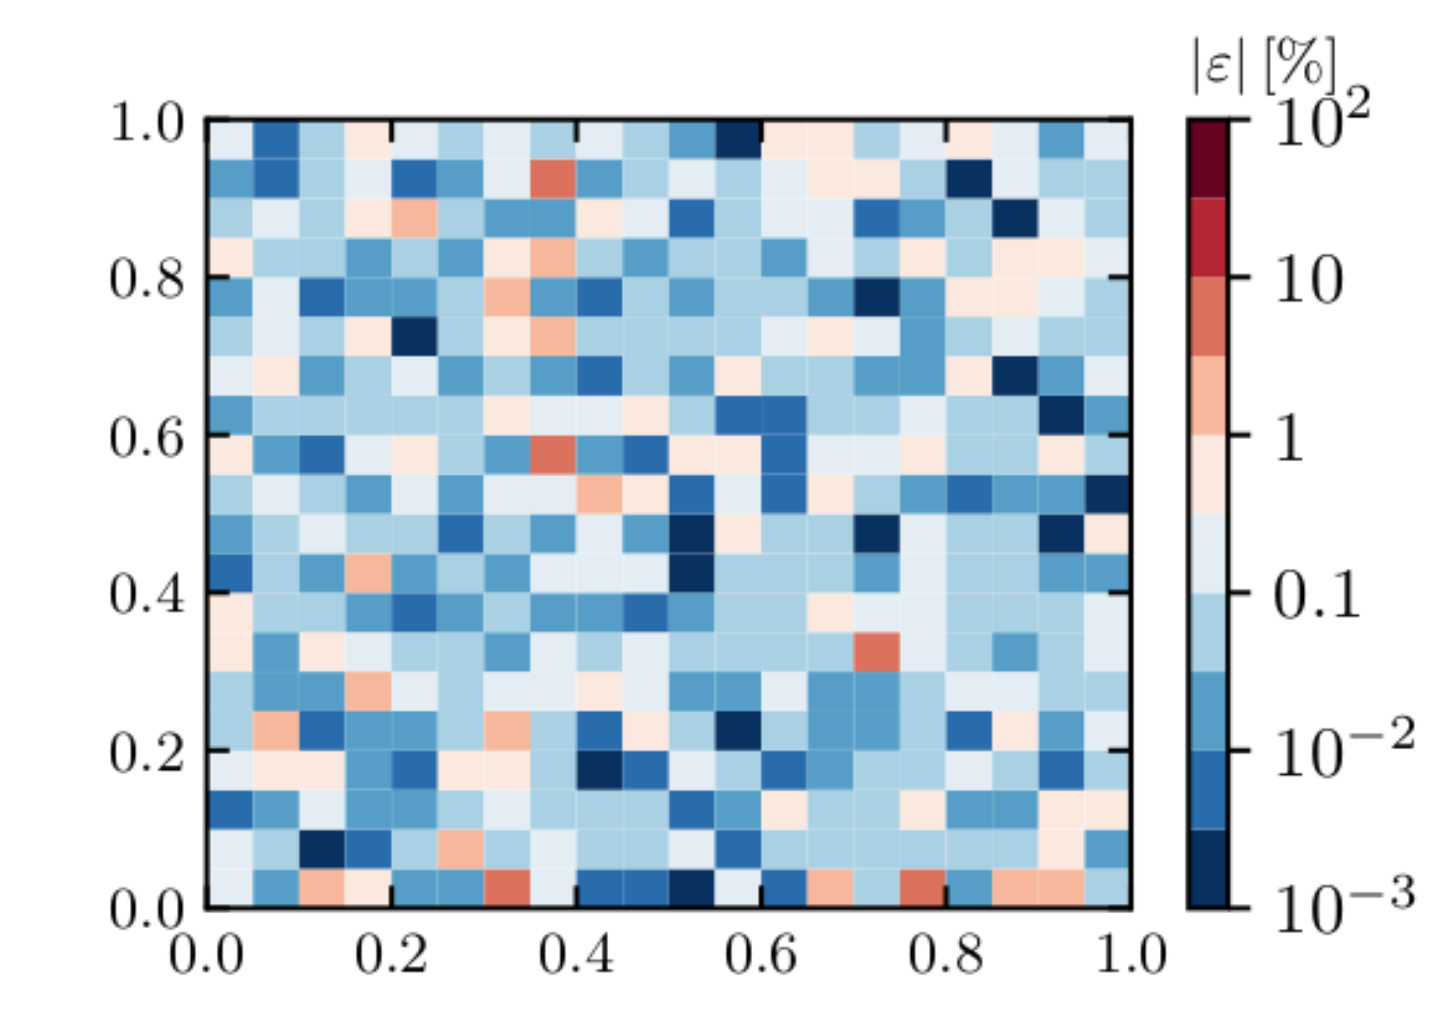
\includegraphics[width=\linewidth]{figs/m3_m4.png}
    \caption{bla bla \red{put correct plot}}
    \label{fig:m3_m4}
\end{figure}


\medskip

%%%%%%%%%%%%%%%%%%%%%%%%%%%%%%%%%%%%%%%%%%%%%%%%%
\section{Summary and conclusions}
\label{sec:Conclusions}

We have shown that ML regressors...
\medskip

There are various other functions that one could try to fit, and this we will do in the future.
\medskip


Also we plan to implement these ML regressors in MATRIX \ref{}.

\medskip

\begin{acknowledgments} 
%\section{Acknowledgments}
\paragraph{\bf Acknowledgements.} We are happy to thank Max Zoller for useful discussions. FB would like to thank the ERC Starting Grant NewAve (638528) and the Deutsche Forschungsgemeinschaft (DFG, German Research Foundation) under Germany's Excellence Strategy – EXC 2121 ``Quantum Universe'' -- 390833306. This research was supported by the Munich Institute for Astro- and Particle Physics (MIAPP) which is funded by the Deutsche Forschungsgemeinschaft (DFG, German Research Foundation) under Germany's Excellence Strategy -- EXC-2094 – 390783311.
\end{acknowledgments}
%

%%%%%%%%%%%%%%%%%%%%%%%%%%%%%%%%%%%%%%%%%%%%%%%%%
%%%%%%%%%%%%%%%%%%%%%%%%%%%%%%%%%%%%%%%%%%%%%%%%%
%%%%%%%%%%%%%%%%%%%%%%%%%%%%%%%%%%%%%%%%%%%%%%%%%
%%%%%%%%%%%%%%%%%%%%%%%%%%%%%%%%%%%%%%%%%%%%%%%%%

%\subsubsection*{Other useful relations}

%The following transformation are combinations of the previous ones in (A.1)-(A.4), and are useful when inferring the helicity amplitudes fitting the least number of regressors as explained in \red{Sec. X}.

%\begin{equation}
%\MAkl{-}{\kappa\lambda} \xrightarrow{\pi_{12}} 
%    (-1)^{N_0+1} \MBkl{-}{\bar{\kappa}\bar{\lambda}} 
%\end{equation}

%\begin{equation}
%{\mathcal{M}^{[A_-]}}_{\kappa\lambda}  \xrightarrow{\pi_{12} \circ \pi_{34}} 
%    (-1)^{N_0} {\mathcal{M}^{[A_-]}}_{\bar{\lambda} \bar{\kappa}} 
%\end{equation}



%%%%%%%%%%%%%%%%%%%%%%%%%%%%%%%%%%%%%%%%%%%%%%%%%%%%%%
%%%%%%%%%%%%%%%%%%%%%%%%%%%%%%%%%%%%%%%%%%%%%%%%%%%%%%
%\subsection{\red{OLD below}} 
%\newcommand{\MRKL}{\mathcal{M}^{[X]}_{r\kappa\lambda}}
%\newcommand{\MArkl}[2]{\mathcal{M}^{[A]}_{#1#2}}
%\newcommand{\MBrkl}[2]{\mathcal{M}^{[B]}_{#1#2}}

%The $q_r\bar{q}_{\bar{r}}\to V_1V_2$ helicity amplitudes $\MRKL$, where $r$ is the helicity of the incoming quark and $\kappa\,(\lambda)$ are the polarizations of $V_1\,(V_2)$, obey the following symmetry properties: \fady{$r=-$ for L and $+$ for R, i.e., it's the eigenvalue of $\gamma_5$}
%\begin{equation}
%\MArkl{-}{\kappa\lambda} \xrightarrow{\pi_{12}} (-1)^{N_0} 
%    \MBrkl{+}{\kappa\lambda}\,,
%\end{equation}
%where $N_0$ is the number of longitudinal polarizations $\kappa,\lambda=0$.
%\begin{equation}
%\MArkl{-}{\kappa\lambda} \xrightarrow{\pi_{34}} 
%   -\MBrkl{-}{\lambda\kappa} 
%\end{equation}
%    
%\begin{equation}
%\MArkl{-}{\kappa\lambda} \xrightarrow{\pi_{12}\circ\pi_{34}} 
%    (-1)^{N_0+1} \MArkl{+}{\lambda\kappa}
%\end{equation}
%%%%%%%%%%%%%%%%%%%%%%%%%%%%%%%%%%%%%%%%%%%%%%%%%%%%%%
%%%%%%%%%%%%%%%%%%%%%%%%%%%%%%%%%%%%%%%%%%%%%%%%%%%%%%

    
%\section{OLD Introduction}

%Need precision for ILC, FCC-ee and CLIC, due to high luminosity, hence need to go to N(N)LO. Problem with time consuming MC generation. Machine learning can solve this, both with phase space integration \cite{} and more recently some works trying to make the evaluation of amplitudes to be faster \cite{Badger:2020uow}. 
%\medskip

%In previous work \cite{} we showed that \xgb can speed up the on loop $gg \to ZZ$ amplitude squared by a factor $\sim 10^3$ with errors in the double differential distribution below $\lesssim 1 \%$. Here we continue that program by studying an NLO process, where more care is needed, in order to deal with the cancellations between the UV and IR divergences between the 1-loop amplitude and the real emission. Also, in this process we have a sharp resonance, which we didn't have in the $gg \to ZZ$ work...
%\medskip

%A hadron colliders it has been shown that diboson processes can be used to improve certain LEP bounds on EW BSM physics, due to their effects growing with the center of mass energy \cite{}....
%\medskip

%
%{\bf The main goal of this work} is to show that we can use ML techniques to compute the relevant amplitudes required to generate $q q \to V_1 V_2$ at NNLO. In particular, we only need to compute the {\it amplitude k-factor} which we define as 
%\begin{equation}
%    K_{n,j}^N = \frac{{\mathcal M}^N_{n+j \, \textrm{loops}}}{{\mathcal M}^N_{n\, \textrm{loops}}}
%\end{equation}
%where ${\mathcal M}_{j}$ stands for a given $2 \to N$ amplitude at $j$ loops. In this work we are interested in computing the {\it amplitude k-factor} with $N=2$, $n=0$ and $j=1$.
%%%%%%%%%%%%%%%%%%%%%%%%%%%%%%%%%%%%%%%%%%%%%%%%%%
%%a%%\section{OLD Theoretical considerations}

%%a%%We can fit all the $2 \to 2$ processes in the NNLO correction, the (1-loop)$^2$ and the interference term (tree $\times $2-loop).

%%a%%The most useful one is the 2-loop interference since it is the slowest. Notice that if we do this, we can not change the EW couplings, because they don't factorize between the different classes A,B,C,F, but obviously we can still factorize $\alpha_s$. To allow for variations in $\alpha_{EW}$, we could either fit benchmark points for it, e.g. $0, M_Z$, or we could fit each class of diagrams A,B,C,F with the SM separately \red{(it seems we would only require the real part, so only 4 pieces to fit?).}

%%a%%\medskip

%%a%%


%%a%%
%%a%%\begin{figure}
%%a%%    \centering
%%a%%    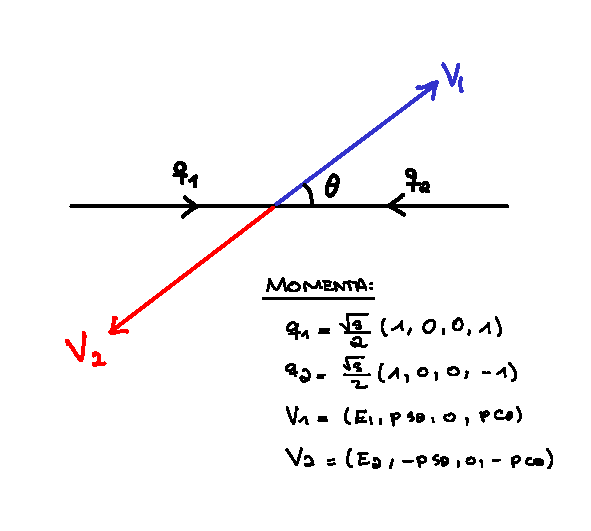
\includegraphics[width=0.5\linewidth]{figs/qq_v1v2_kin.pdf}
%%a%%    \caption{Kinematic configuration and definition of the polar angle $\theta$.}
%%a%%    \label{fig:kinematics}
%%a%%\end{figure}

%%a%%\subsection{Off-shell matrix elements}

%%a%%The scattering angle when both $Z$s are off-shell with invariant masses $m_1$ and $m_2$ is given by

%%a%%\begin{equation}
%%a%%    %\cos\theta = \frac{1}{\shat\lambda}\left(2t+\shat-m_1^2-m_2^2\right)\,,
%%a%%    \cos\theta = \frac{t-u}{\shat\lambda}\,,
%%a%%\end{equation}
%%a%%where $\lambda$ is the triangle (a.k.a. K{\"a}ll{\'e}n) function defined as
%%a%%\begin{equation}
%%a%%    \lambda\equiv\sqrt{(1+x+y)(1-x-y)(1+x-y)(1-x+y)}\,.
%%a%%\end{equation}
%%a%%Here, $x=m_1/\rtshat$ and $y=m_2/\rtshat$.
%%a%%%%%%%%%%%%%%%%%%%%%%%%%%%%%%%%%%%%%%%%%%%%%%%%%%%
%%a%%\section{ML Algorithm and training}

%%a%%To train and test the \xgb regressor, we generate \red{X} million (\red{XM}) pairs of phase space points $(\sqrt{\hat{s}},\cos \theta)$ uniformly distributed in the region defined by,
%%a%%\begin{equation}
%%a%%\begin{split}
%%a%%\sqrt{\hat{s}} &\in [2\sqrt{\mz^2+\ptx^2}, 3 \, \mathrm{TeV}] \,,\\
%%a%%\cth &\in [-1,1]\times \sqrt{1-\frac{4p_T^\text{cut}}{\hat{s}-4\mz^2}}\,,
%%a%%\label{eq:PSregion}
%%a%%\end{split}
%%a%%\end{equation}
%%a%%%
%%a%%with \red{$p_T^\text{cut} = 1$} GeV to regulate the singularity in $\msq$ in the limit $p_T \rightarrow 0$ (similarly to what is done in \texttt{MCFM} \cite{Campbell:2010ff} and \texttt{Madgraph\_aMC@NLO} \cite{Hirschi:2015iia}). \red{We choose  $(\sqrt{\hat{s}} \, )_{max}$ = 3 TeV as an arbitrary cutoff relevant for LHC physics. Nonetheless, it is straightforward to increase it (see Section \ref{sec:accNspeed}).}

%%a%%
%%a%%\section{Form factors}
%%a%%From Fig.~\ref{fig:kinematics} we have:
%%a%%\begin{eqnarray}
%%a%%p_1^\mu &=& \frac{\sqrt{s}}{2} \, (1, \, 0, \, 0, \, 1) \\
%%a%%p_2^\mu &=& \frac{\sqrt{s}}{2} \, (1, \, 0, \, 0, \, -1) \\
%%a%%p_3^\mu &=& \frac{\sqrt{s}}{2} \,  (1, \, r \, \sin \theta, \, 0, \, r \, \cos \theta) \\
%%a%%p_4^\mu &=& \frac{\sqrt{s}}{2} \,  (1, \, - r \, \sin \theta, \, 0, \, - r \, \cos \theta) 
%%a%%\end{eqnarray}
%%a%%\smallskip

%%a%%where $r = \sqrt{1 - 4 M_Z^2/s}$.
%%a%%\medskip

%%a%%The polarizations are: \red{need to check}
%%a%%\begin{eqnarray}
%%a%%    \left[\epsilon_3^\mu (p_3)^*\right]_+ &=& \frac{1}{\sqrt{2}} (0, \, \cos \theta, \, i , \, - \sin \theta) \\
%%a%%    \left[\epsilon_3^\mu (p_3)^*\right]_- &=& \frac{1}{\sqrt{2}} (0, \, -\cos \theta, \, i , \,  \sin \theta) \\
%%a%%    \left[\epsilon_3^\mu(p_3)^*\right]_0 &=& \frac{\sqrt{s}}{2 M_Z} (r, \, \sin \theta, \, 0 , \,  \cos \theta) \\
%%a%%    \left[\epsilon_4^\mu (p_4)^*\right]_+ &=& \frac{1}{\sqrt{2}} (0, \, -\cos \theta, \, i , \,  \sin \theta) \\
%%a%%    \left[\epsilon_4^\mu (p_4)^*\right]_- &=& \frac{1}{\sqrt{2}} (0, \, \cos \theta, \, i , \,  -\sin \theta) \\
%%a%%    \left[\epsilon_4^\mu(p_4)^*\right]_0 &=& \frac{\sqrt{s}}{2 M_Z} (-r, \, \sin \theta, \, 0 , \,  \cos \theta)
%%a%%\end{eqnarray}
%%a%%\medskip

%%a%%We define the massles spinors in the Weyl basis. From Peskin p. 46, Eq.~(3.50):
%%a%%\begin{equation}
%%a%%    u(p)=\left(\begin{array}{ll} U_L(p) \\ U_R(p) \end{array}\right) = \left(\begin{array}{ll}\sqrt{p^0 \sigma_0- p^i \sigma_i} & \xi \\ \sqrt{p^0 \sigma_0 + p^i \sigma_i} & \xi \end{array}\right)
%%a%%\end{equation}

%%a%%The spinors for massless quarks are:
%%a%%\begin{eqnarray}
%%a%%    u_L(p_1) &=& s^{1/4} (0, \, 1, \, 0, \, 0)^T \\
%%a%%    u_R(p_1) &=& s^{1/4} (0, \, 0, \, 1, \, 0)^T \\
%%a%%    u_L(p_2) &=& s^{1/4} (1, \, 0, \, 0, \, 0)^T \\
%%a%%    u_R(p_2) &=& s^{1/4} (0, \, 0, \, 0, \, 1)^T 
%%a%%\end{eqnarray}

%%a%%hence
%%a%%\begin{eqnarray}
%%a%%    u(p_1) &=& s^{1/4} (0, \, 1, \, 1, \, 0)^T \\
%%a%%    u(p_2) &=& s^{1/4} (1, \, 0, \, 0, \, 1)^T \\
%%a%%\end{eqnarray}

%%a%%Finally the last piece we need:
%%a%%\begin{eqnarray}
%%a%%    \bar{u}_L(p_2) &=& \left[u_L(p_2)\right]^\dagger \gamma_0 = s^{1/4} (0, \, 0, \, 1, \, 0) \\
%%a%%    \bar{u}_R(p_2) &=& \left[u_R(p_2)\right]^\dagger \gamma_0 = s^{1/4} (0, \, 1, \, 0, \, 0) 
%%a%%\end{eqnarray}
%%a%%hence
%%a%%\begin{eqnarray}
%%a%%    \bar{u}(p_2) &=& s^{1/4} (0, \, 1, \, 1, \, 0)
%%a%%\end{eqnarray}

%%a%%The only form factors needed for the SM inteference are:
%%a%%\begin{equation}
%%a%%\begin{array}{ll}
%%a%%T^{(7)}_{\mu \nu}=\bar{u}\left(p_{2}\right) \gamma_{\nu} u\left(p_{1}\right) p_{1 \, \mu}, 
%%a%%& 
%%a%%T^{(8)}_{\mu \nu}=\bar{u}\left(p_{2}\right) \gamma_{\nu} u\left(p_{1}\right) p_{2\, \mu} \\
%%a%%%
%%a%%T^{(9)}_{\mu \nu}=\bar{u}\left(p_{2}\right) \gamma_{\mu} \not p_{3} \gamma_{\nu} \, u\left(p_{1}\right),
%%a%%& 
%%a%%T^{(10)}_{\mu \nu}=\bar{u}\left(p_{2}\right) \gamma_{\nu} \not p_{3} \gamma_{\mu} \, u\left(p_{1}\right)
%%a%%\end{array} \nonumber
%%a%%\end{equation}
%%a%%%%%%%%%%%%%%
%%a%%\newpage
%%a%%%%%%%%%%%%%%%

%%a%%Defining $S^{(i)} = \sum_{i,j} T^{(i)}_{\mu \nu} \left[\epsilon_3^\mu (p_3)^*\right]_i \left[\epsilon_4^\nu (p_4)^*\right]_j$ we find that:
%%a%%\begin{eqnarray}
%%a%%   S^{(7)} &=& \frac{\sqrt{2} s (r-\cos (\theta ))}{\sqrt{1-r^2}} \,,\\
%%a%%   S^{(8)} &=& \frac{\sqrt{2} s (r-\cos (\theta ))}{\sqrt{1+r^2}} \,, \\
%%a%%   S^{(9)} &=& -\frac{2 \sqrt{2} r s (r \cos (\theta )-1)}{\sqrt{1-r^2}} \,,\\
%%a%%   S^{(10)} &=&  \frac{2 \sqrt{2} r s (r \cos (\theta )+1)}{\sqrt{1-r^2}} \,,
%%a%%\end{eqnarray}
%%a%%where remember that $r = \sqrt{1 - 4 M_Z^2/s}$.

%%a%%\newpage
%%%%%%%%%%%%%%%%%%%%%%%%%%%%%%%%%%%%%
\bibliography{paper}
%%%%%%%%%%%%%%%%%%%%%%%%%%%%%%%%%%%%%
\end{document}
%%%%%%%%%%%%%%%%%%%%%%%%%%%%%%%%%%%%%
%%%%%%%%%%%%%%%%%%%%%%%%%%%%%%%%%%%%%
%%%%%%%%%%%%%%%%%%%%%%%%%%%%%%%%%%%%%
%%%%%%%%%%%%%%%%%%%%%%%%%%%%%%%%%%%%%
